
\section{Auswertung}
Vor Beginn der Messung wurde zunächst der Dunkelstrom gemessen.
Dieser beträgt
\begin{equation*}
  I_{Dunkel} = 5\, \si{\nano\ampere}
\end{equation*}
und muss von den gemessenen Stromwerten abgezogen werden.\\
Der ausgemessene Abstand zwischen Spalt und Detektor beträgt
  $L_1 = 99,05\, \si{\centi\meter}$.
Der Abstand zwischen dem Laser und dem Spalt beträgt
$  L_2= 5,95\, \si{\centi\meter}$.
\subsection{Einzelspalt 0.075 mm}

In Tabelle (\ref{tab:e75}) sind die gemessenen Werte für einen Einzelspalt
 mit einer Spaltbreite von $b=0,075\, \si{\milli\meter}$ zu finden.
 In allen Tabellen sind die gemessenen Werte ohne Abzug des Dunkelstroms zu sehen.
 Zum erstellen der Graphen wurde dieser allerdings berücksichtigt.
\begin{table}
  \centering
  \caption{Einzelspalt 0,075mm}
  \label{tab:e75}
  \begin{tabular}{c c|| c c}
    \toprule
    $\symup{Abstand}$/ \si{\micro\meter} & $\symup{Strom}$ / \si{\nano\ampere}
    & $\symup{Abstand}$/ \si{\micro\meter} & $\symup{Strom}$ / \si{\nano\ampere}\\
    \midrule
    3   & 7,2 & 24  & 9\\
    6   & 7,2 & 25  & 5,6\\
    6,5 & 7,6 & 27  & 13,5\\
    7   & 7,8 & 28  & 11\\
    7,5 & 8,2 & 29  & 16\\
    8   & 9   & 29,5& 19,5\\
    8,5 & 9,4 & 30  & 22,5\\
    9   & 10  & 30,5& 24\\
    9,5 & 10  & 31  & 25\\
    11  & 9,8 & 31,5& 24,5\\
    11,5& 9,2 & 32  & 22,5\\
    12  & 8,4 & 33  & 17\\
    13  & 7,6 & 34  & 11,5\\
    14  & 9,8 & 35  & 8,2\\
    15  & 17,5& 36  & 8\\
    16  & 34  & 36,5& 9\\
    18  & 10  & 37  & 10\\
    19  & 13  & 37,5& 11\\
    20  & 15,5& 38  & 11,5\\
    20,5& 16,5& 38,5& 115\\
    21  & 16,5& 39  & 11\\
    22  & 16  & 39,5& 10\\
    22,5& 15 & & \\
    \bottomrule
  \end{tabular}
\end{table}

Eine Regression wurde mit der Formel (\ref{eqn:reg})
%\begin{equation}
%  I(\varphi) = I_0^2 b^2\left(\frac{\lambda}{\pi b sin(\varphi)}\right)^2 \cdot sin\left(\frac{\pi b sin(\varphi)}{\lambda}\right)
%\label{eqn:reg}
%\end{equation}
durchgeführt.\\
%Hierbei ist $I_0$ die Amplitude und b die Spaltbreite.
%Der Beugungswinkel $\varphi$ ergibt sich durch $\frac{(x-x0)}{L_1}$.
Die Wellenlänge $\lambda$ des Lasers wurde aus der Anleitung entnommen und beträgt $633\, \mathrm{nm}$.\\
%Die Regression wurden für zwei unterschiedliche Mittelpunkte durchgeführt.
%Zum einen bei $20,5\, \mathrm{mm}$, wo er auch bei den anderen beiden Spalten liegt und vermutet wurde,
Der Mittelpunkt liegt bei $31\, \mathrm{mm}$. Dieser Wert wurde aus den Messwerten entnommen.\\
aus dem Graphen wurden zwei Punkte herausgenommen,
da diese sehr weit von der vermuteten Verteilung wegliegen und somit fehlerhaft sein müssen.
Auf mögliche Fehlerquellen wird genauer in der Diskussion eingegangen.\\
%In Abbildung (\ref{fig:e75}) ist die Regression für eine Verschieung um $20,5\, \mathrm{mm}$ zu sehen.
%\begin{figure}[H]
%\centering
%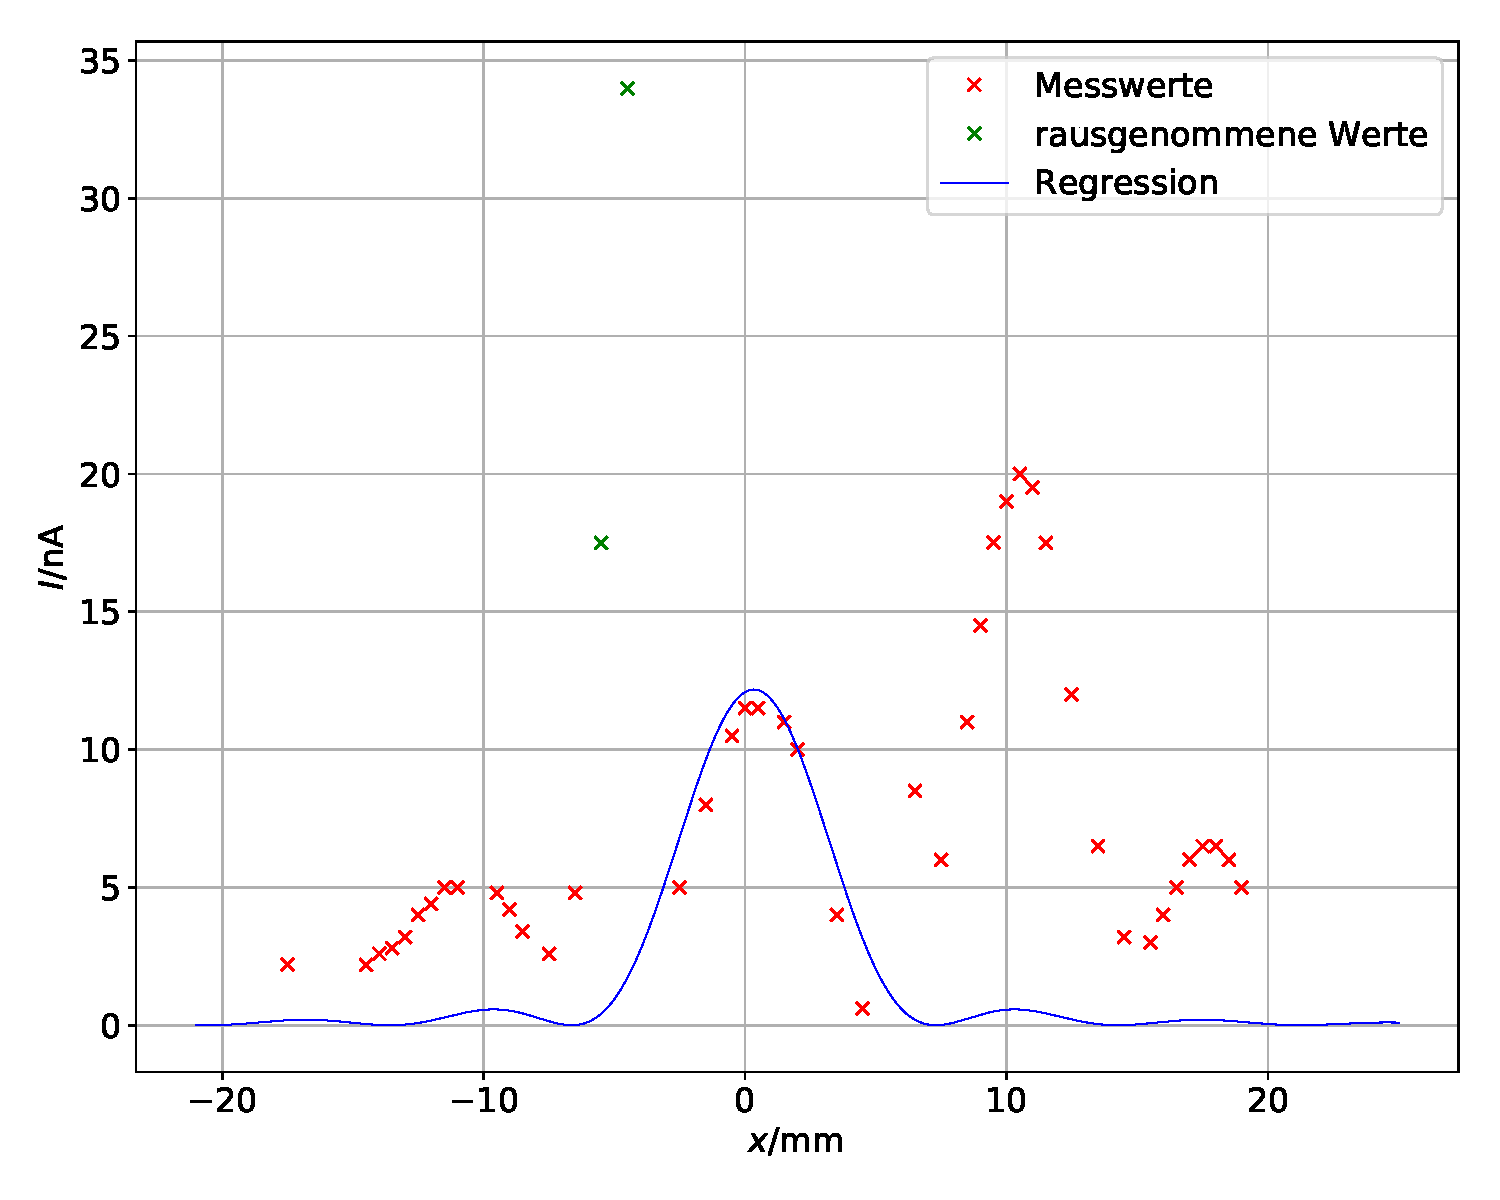
\includegraphics[width=\textwidth]{einzel75.pdf}
%\caption{1. Einzelspalt 0,075mm}
%\label{fig:e75}
%\end{figure}
%Es ergibt sich  eine Spaltbreite von
%\begin{equation*}
%  b= (0,090 \pm 0,043)\, \mathrm{mm}
%\end{equation*}
%Das entspricht einer Abweichung von $20\%$ zu der tatsächlichen Spaltbreite.\\
%Wird nun der Mittelunkt auf $31\, \mathrm{mm}$ gelegt ergibt sich die Abbildung (\ref{fig:e752}).
Die Regression ist in Abbilung (\ref{fig:e752}) zu sehen.
\begin{figure}[H]
\centering
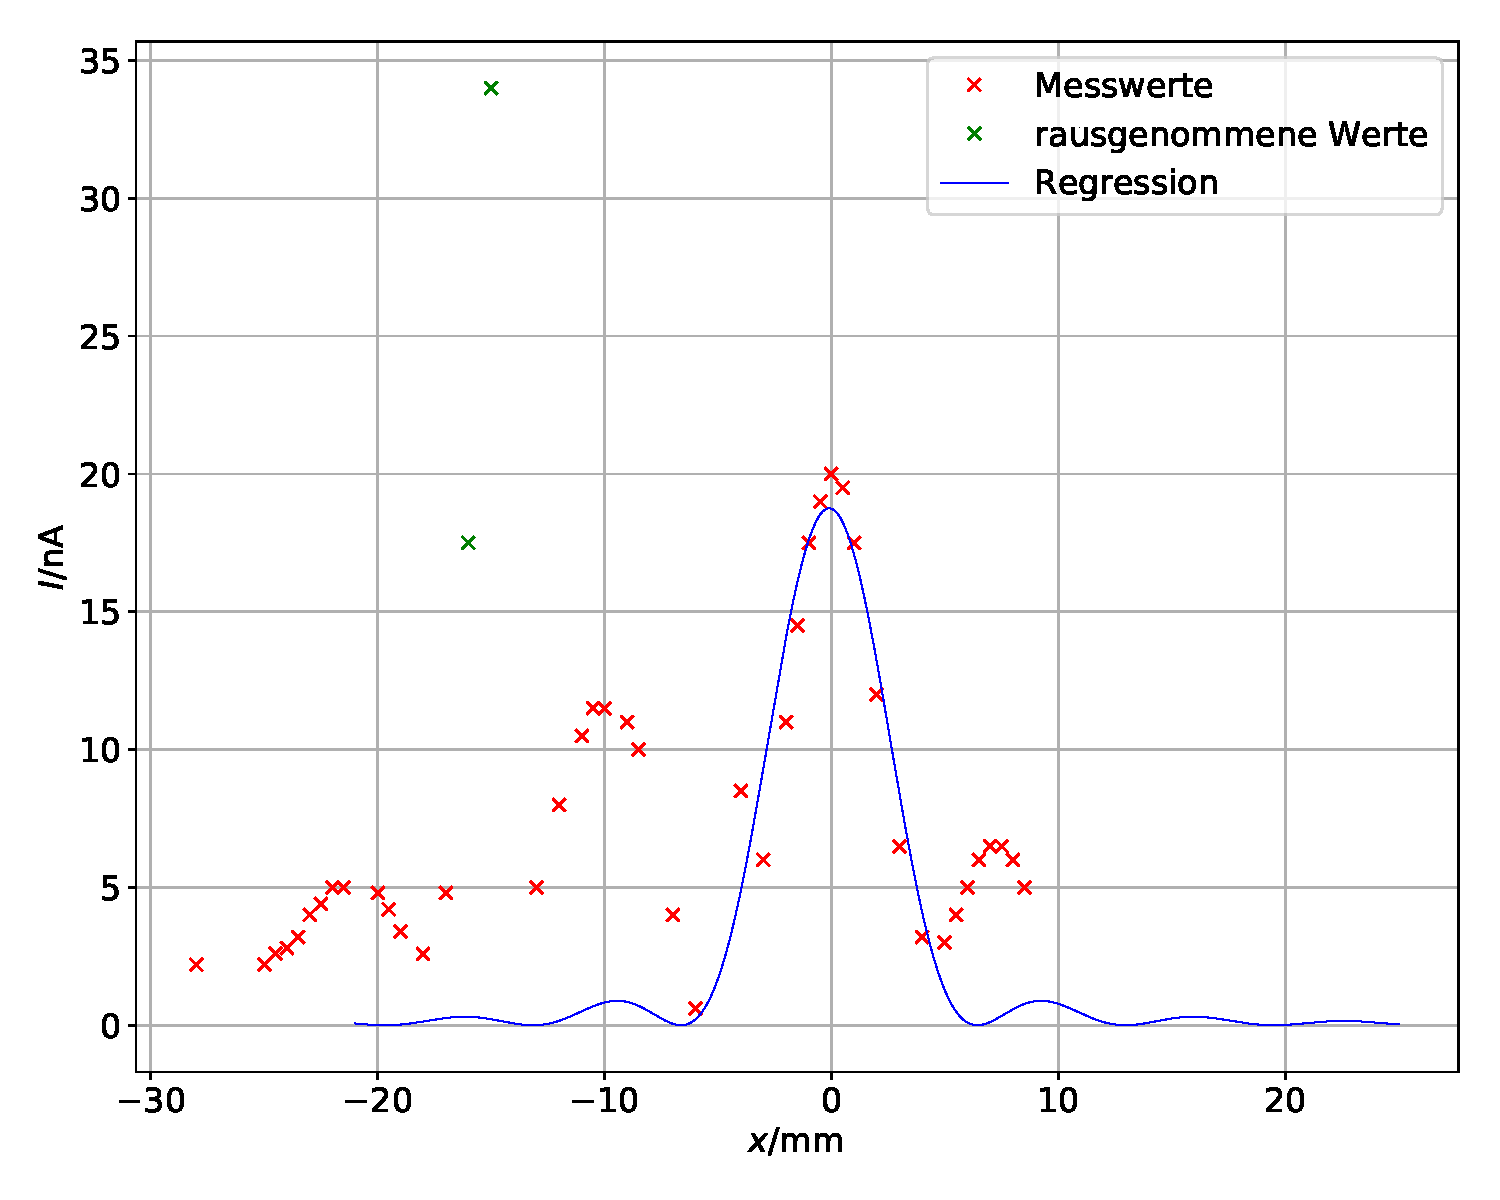
\includegraphics[width=\textwidth]{test2.pdf}
\caption{2. Einzelspalt 0,075mm}
\label{fig:e752}
\end{figure}
Hier ergibt sich eine Spaltbreite von
\begin{equation*}
  b= (0,096 \pm 0,015)\, \mathrm{mm}
\end{equation*}
Die prozentuale Abweichung zur tatsächlichen Spaltbreite beträgt $28\%$.

\newpage
\subsection{Einzelspalt 0.15 mm}
Tabelle (\ref{tab:e15}) zeigt die gemessenen Werte für eine Spaltbreite von
$b=0,15\, \mathrm{mm}$.

\begin{table}[H]
  \centering
  \caption{Einzelspalt 0,15mm}
  \label{tab:e15}
  \begin{tabular}{c c|| c c}
    \toprule
    $\symup{Abstand}$/ \si{\micro\meter} & $\symup{Strom}$ / \si{\nano\ampere}
    & $\symup{Abstand}$/ \si{\micro\meter} & $\symup{Strom}$ / \si{\nano\ampere}\\
    \midrule
    9    & 9,2  & 24   & 25\\
    10   & 11   & 24,5 & 13,5\\
    10,5 & 12,5 & 25   & 20,5\\
    11   & 13,5 & 25,5 & 32\\
    11,5 & 13   & 26   & 36\\
    12   & 11,5 & 26,5 & 34\\
    13   & 10,5 & 27   & 26\\
    13,5 & 15   & 28   & 13,5\\
    14   & 22,5 & 28,5 & 14,5\\
    14,5 & 30   & 29   & 18\\
    15   & 34   & 29,5 & 22\\
    15,5 & 30   & 30   & 21\\
    16   & 21,5 & 30,5 & 18,5\\
    17   & 20   & 31   & 14,5\\
    18   & 125  & 32   & 10,5\\
    19   & 360  & 32,5 & 12,5\\
    19,5 & 480  & 33   & 15,5\\
    20   & 600  & 33,5 & 17,5\\
    20,5 & 620  & 34   & 17,5\\
    21   & 600  & 34,5 & 15\\
    21,5 & 520  & 35   & 11,5\\
    22   & 400  & 36   & 8,2\\
    23   & 150  & & \\
  \bottomrule
  \end{tabular}
\end{table}
Für diese Werte wurde ebenfalls eine Regression mit der Formel (\ref{eqn:reg}) durchgeführt.
Sie ist in Abblidung (\ref{fig:e15}) zusehen.
Der Mittelpunkt liegt bei $20,5\, \mathrm{mm}$.
\begin{figure}[H]
\centering
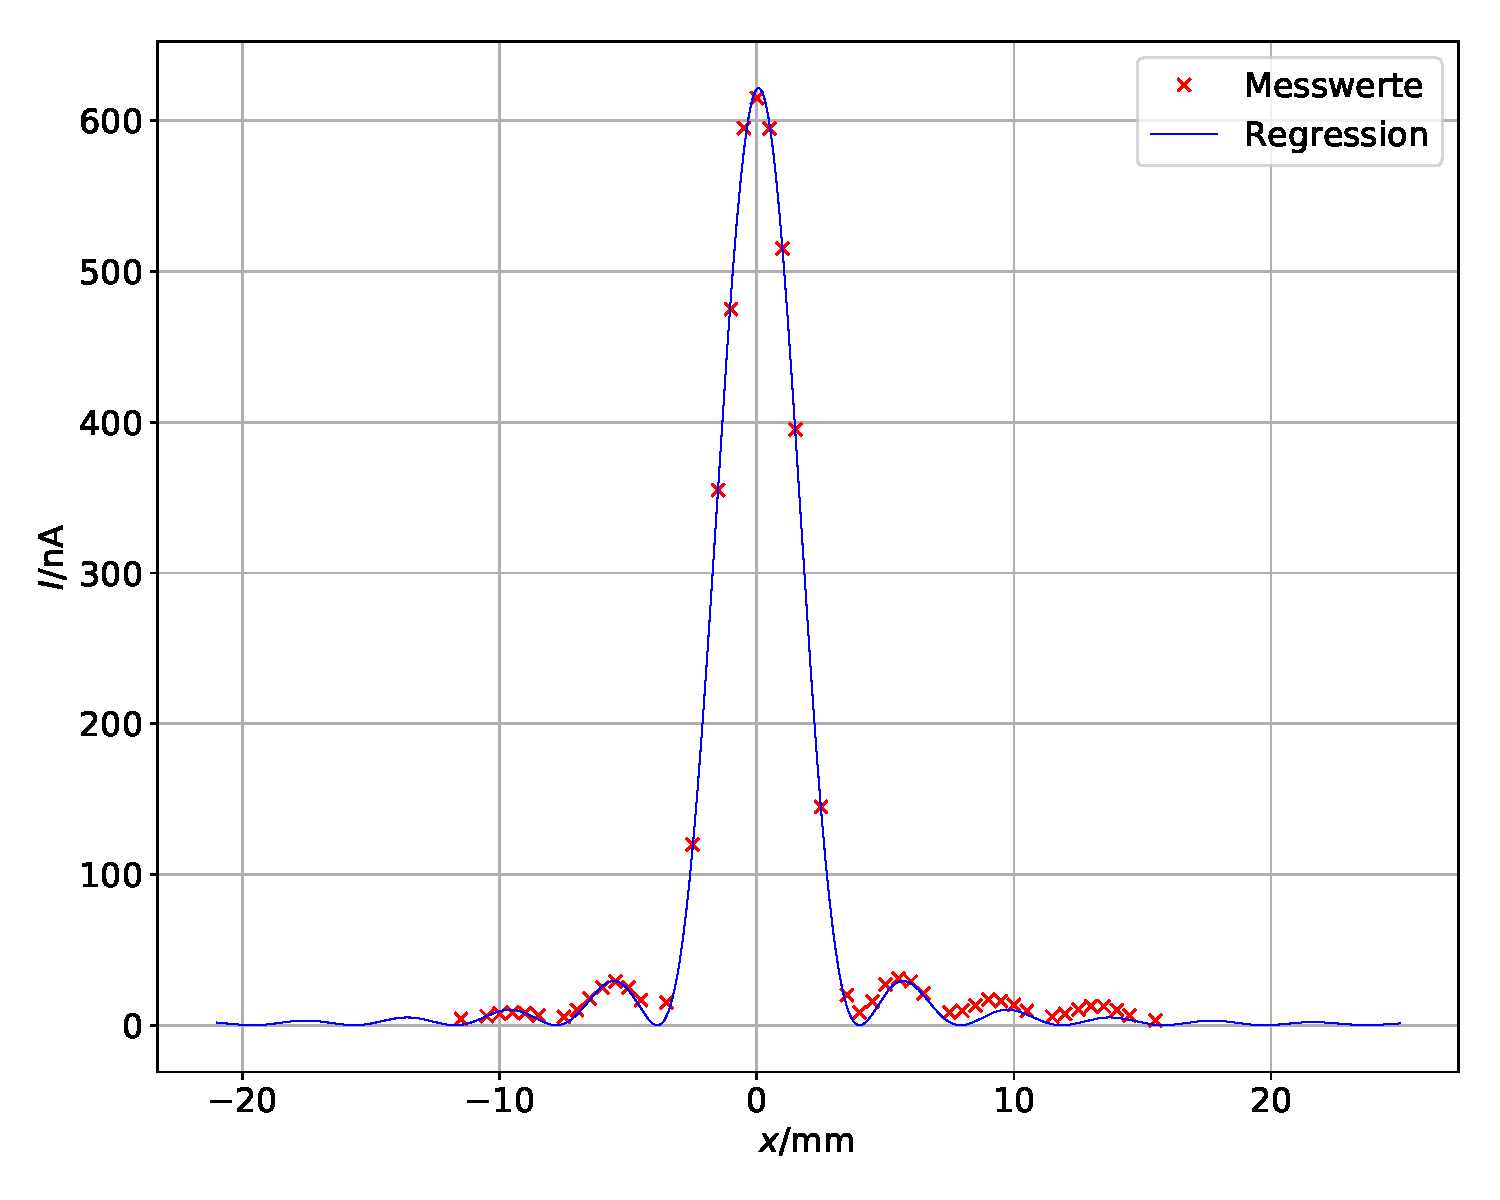
\includegraphics[width=\textwidth]{einzel15.pdf}
\caption{Einzelspalt 0,15mm}
\label{fig:e15}
\end{figure}
Aus der Regression ergibt sich die experimentell bestimmte Spaltbreite.
\begin{equation*}
  b = (0,15939 \pm 0,00104)\, \mathrm{mm}
\end{equation*}
Dies entspricht einer Abweichung von $6,26\%$ zum angegebenen Wert.
\newpage
\subsection{Doppelspalt}

In Tabelle(\ref{tab:dop}) werden die Werte für einen Doppelspalt mit der Spaltbreite $b= 0,15\, \mathrm{mm}$
und dem Spaltabstand $s= 0,5\, \mathrm{mm}$ aufgelistet.
\begin{table}[H]
  \centering
  \caption{Doppelspalt}
  \label{tab:dop}
  \begin{tabular}{c c || c c}
    \toprule
    $\symup{Abstand}$/ \si{\micro\meter} & $\symup{Strom}$ / \si{\micro\ampere}
    & $\symup{Abstand}$/ \si{\micro\meter} & $\symup{Strom}$ / \si{\micro\ampere}\\
    \midrule
    9     & 0,0155 & 19,5  & 0,86\\
    10    & 0,0105 & 20    & 1\\
    10,5  & 0,001  & 20,5  & 1,5\\
    10,75 & 0,0145 & 21    & 0,74\\
    11    & 0,021  & 21,5  & 1,2\\
    11,25 & 0,0235 & 22    & 0,5\\
    11,5  & 0,0185 & 22,5  & 0,44\\
    12    & 0,18   & 23    & 0,26\\
    12,25 & 0,0255 & 24    & 0,04\\
    12,5  & 0,028  & 25    & 0,07\\
    12,75 & 0,025  & 25,5  & 0,046\\
    13    & 0,0205 & 26    & 0,07\\
    14    & 0,0275 & 27    & 0,026\\
    14,25 & 0,034  & 28    & 0,018\\
    14,5  & 0,054  & 29    & 0,022\\
    14,75 & 0,052  & 29,5  & 0,032\\
    15    & 0,036  & 30    & 0,024\\
    15,5  & 0,048  & 30,5  & 0,018\\
    15,75 & 0,056  & 31    & 0,012\\
    16    & 0,052  & 32    & 0,02\\
    17    & 0,058  & 32,5  & 0,018\\
    18    & 0,36   & 33    & 0,024\\
    18,5  & 0,28   & 33,5  & 0,018\\
    19    & 0,94   & 34    & 0,014\\
  \bottomrule
  \end{tabular}
\end{table}
In Abbildung (\ref{fig:dop}) sind die gemessenen Werte für den Doppelspalt,
sowie eine darüber gelegte Theoriekurve zu sehen.
Außerdem ist ebenfalls die Kurve für den Einzelspalt mit $0,15\, \mathrm{mm}$ Breite
aufgetragen.\\
Die Ausgleichsfunktion wurde mit Formel (\ref{eqn:aus}) bestimmt.
%\begin{equation*}
%  I(\varphi) = 4cos^2\left(\frac{\pi s \cdot sin\varphi}{\lambda}\right)\cdot
%  \left(\frac{\lambda}{\pi b sin\varphi}\right)^2
%  \cdot sin^2\left(\frac{\pi b sin\varphi}{\lambda}\right)
%\end{equation*}
\begin{figure}
\centering
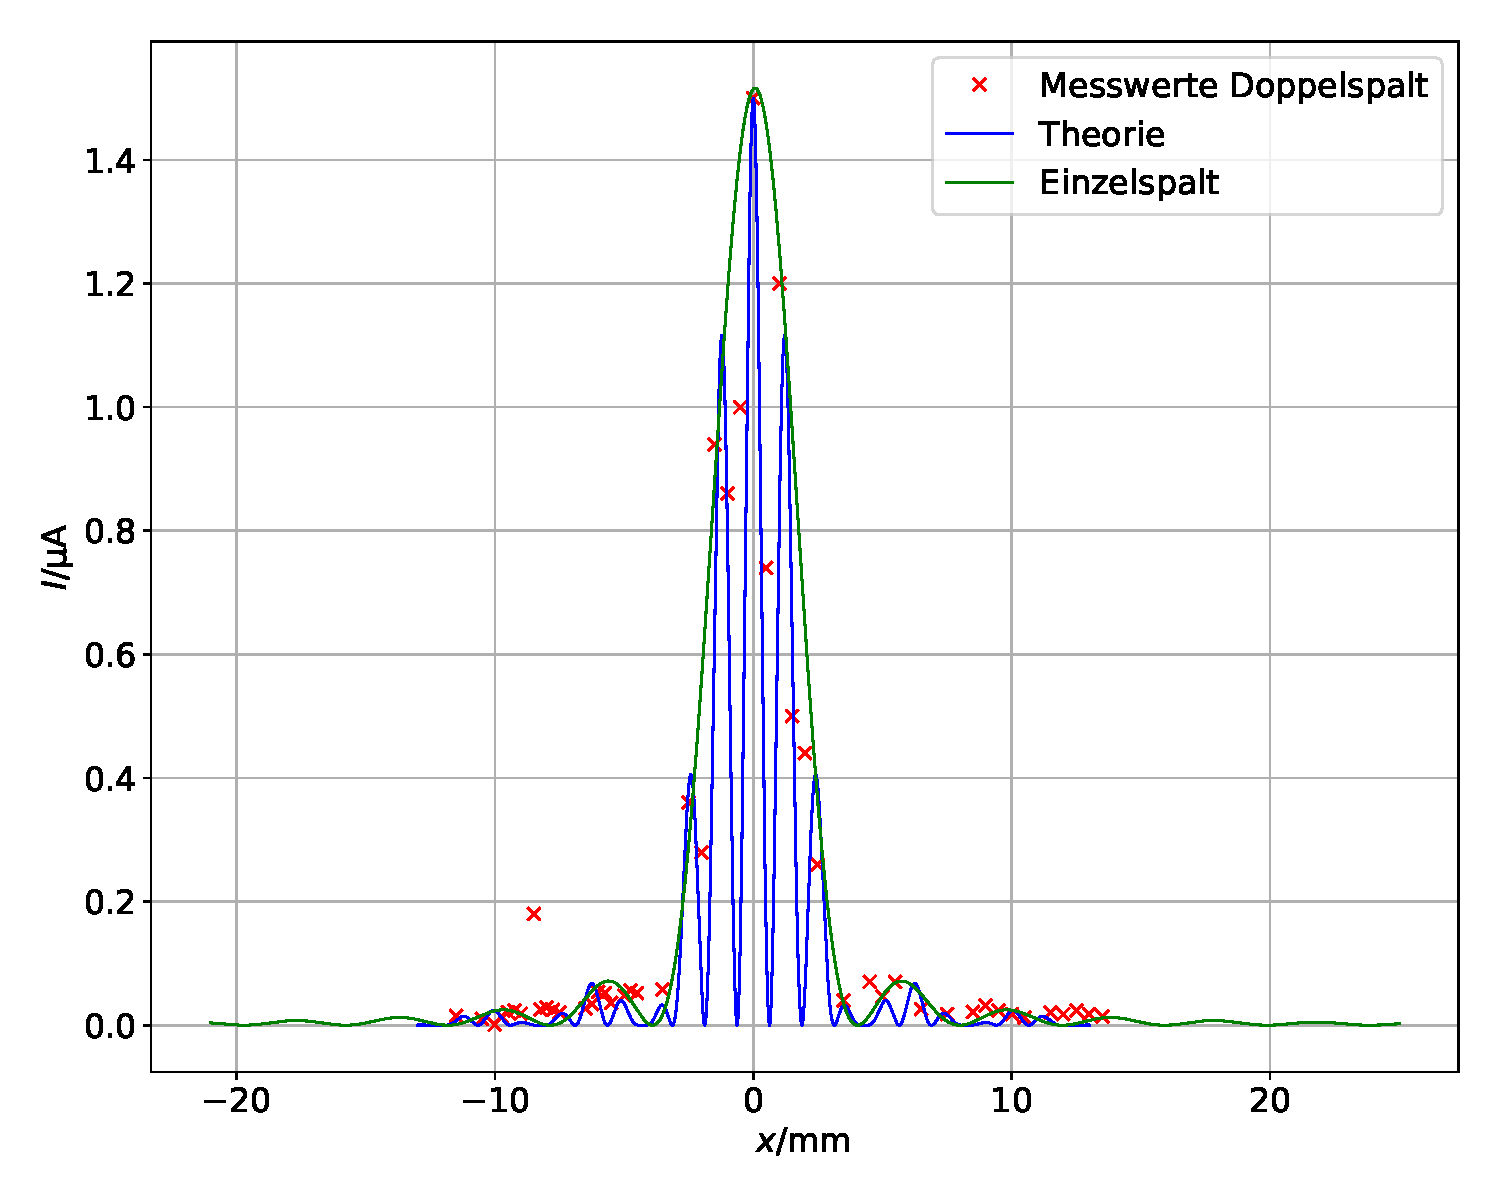
\includegraphics[width=\textwidth]{doppel2.pdf}
\caption{Der Doppelspalt}
\label{fig:dop}
\end{figure}
Die Kurve des Einzelspaltes wurden mit dem Faktor 413,3
an die des Doppelspaltes angepasst um diese aufeinander legen zu können.
Auf den Vergleich wird in der Diskussion eingegangen.


\section{Diskussion}
Bei der ersten Messung muss es zu einem Fehler gekommen sein.
Es gibt zwei Messwerte die nicht ins Bild passen, zudem ist das Interferenzmuster nicht klar erkennbar.
Wo dieser Fehler lag kann nicht mehr genau nachvollzogen werden.
Zu möglichen Fehlerquellen gehört zum einen das Lichtverhältnis im Versuchsraum.
Diese waren nicht konstant, da mehrere Personen in diesem Raum gearbeitet haben.
Somit ist der Dunkelstrom nicht genau messbar.\\
Bei der nächsten Messung wurden die Messwerte viel genauer.
Der einzige Unterschied zur vorherigen Messung lag darin,
dass vor Beginn der Messung die ungefähre Stellung und der Strom der einzelen Hochpunkte notiert wurde.
Es ist zuerkennen, dass die Maxima mit größer werdender Spaltbreite schmaler werden,
was dem Verhalten des Beugungsmusters des Einzelspaltes entspricht.\\
Bei der Messung des Doppelspaltes wurden die Messwerte nicht eng genug genommen.
Dies führt dazu, dass das Interferenzmuster nicht genau erkennbar ist,
auch wenn die Punkte alle ungefähr auf der Ausgleichsfunktion liegen.
Es ist gut zu erkennen, dass die Messwerte des Einzelspaltes eine einhüllende Kurve ergeben.
Durch die Überlagerung der Wellen, entsteht ein Wellenpaket.
In dem Hauptmaxima des Einzelspaltes sind mehrere Maxima des Doppelspalte eingeschlossen.\\
Der angegebene Abstand zwischen Spalt und Detektor wurde am Versuchstag vergessen zu messen.
Dies wurde am darauf folgenden Tag nachgeholt.
Es ist allerdings nicht sicher, ob innerhalb des Tages die Apparatur verändert wurde.
